\documentclass[zavrsnirad]{fer}
% Dodaj opciju upload za generiranje konačne verzije koja se učitava na FERWeb
% Add the option upload to generate the final version which is uploaded to FERWeb


\usepackage{blindtext}


%--- PODACI O RADU / THESIS INFORMATION ----------------------------------------

% Naslov na engleskom jeziku / Title in English
\title{Development of an agent for solving the Entaglement game}

% Naslov na hrvatskom jeziku / Title in Croatian
\naslov{Razvoj agenta za igranje igre Entanglement}

% Broj rada / Thesis number
\brojrada{1}

% Autor / Author
\author{Iva Rengel}

% Mentor 
\mentor{Prof.\@ Marko Đurasević}

% Datum rada na engleskom jeziku / Date in English
\date{June, 2024}

% Datum rada na hrvatskom jeziku / Date in Croatian
\datum{lipanj, 2024.}

%-------------------------------------------------------------------------------


\begin{document}


% Naslovnica se automatski generira / Titlepage is automatically generated
\maketitle


%--- ZADATAK / THESIS ASSIGNMENT -----------------------------------------------

% Zadatak se ubacuje iz vanjske datoteke / Thesis assignment is included from external file
% Upiši ime PDF datoteke preuzete s FERWeb-a / Enter the filename of the PDF downloaded from FERWeb
\zadatak{filename.pdf}


%--- ZAHVALE / ACKNOWLEDGMENT --------------------------------------------------

\begin{zahvale}
  % Ovdje upišite zahvale / Write in the acknowledgment
  Hvala na kavi...
\end{zahvale}


% Odovud započinje numeriranje stranica / Page numbering starts from here
\mainmatter


% Sadržaj se automatski generira / Table of contents is automatically generated
\tableofcontents


%--- UVOD / INTRODUCTION -------------------------------------------------------
\chapter{Uvod}
\label{pog:uvod}

Neki od radova koje ćemo citirati su \cite{6248073,6247753,ghiglia_pritt_phase_unwrapping,hartley2003multiple,4250461,123DCatch}.
Trebaju nam samo radi testiranja kako izgleda referenciranje rada s konferencije, rada iz časopisa, knjige i Internetske stranice.

\begin{figure}[htb]
  \centering
  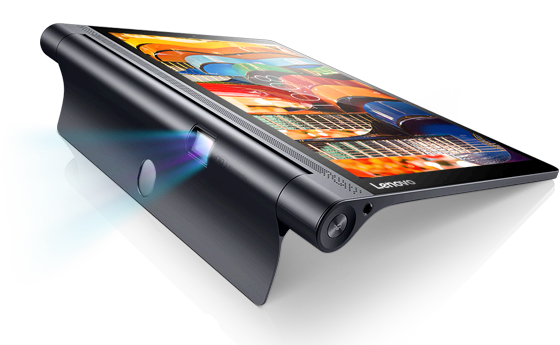
\includegraphics[width=0.38\linewidth]{Figures/lenovo_yoga_tab3_pro_front.png} 
  \caption{Moja prva slika}
  \label{slk:prvaslika}
\end{figure}

Referenciramo se na sliku \ref{slk:prvaslika} u sredini rečenice, zatim prije zareza \ref{slk:prvaslika}, te zatim na kraju rečenice \ref{slk:prvaslika}.
Upravo smo testirali radi li naredba \verb|\ref| ispravno u slučaju kada nakon nje slijedi točka.

Sada slijedi jedna jednadžba:
\begin{equation}
  \label{jed:prvajednadzba}
  \int_{-\infty}^{+\infty}f(t)\,dt=F(\omega)
\end{equation}
Jednadžba \eqref{jed:prvajednadzba} je moja prva jednadžba koja defnira par $f(t)\ufrek F(\omega)$ ili $F(\omega)\uvrem f(t)$.

Opis zadatka gdje ce se pojaviti ovaj tekst? Neznam dok ne convertam opet PDF? Tocno.
Okay, krenimo s pisanjem zavrsnog.

Poručiti pravila igranje igre Entaglement. Razviti jednostavno programsko okruženje koje omogućuje testiranje različitih agenata za igranje navedene igre. Razviti jednostavne heuristike za igranje navedene igre. Proučiti literaturu koja se bavi razvojem agenata za slične probleme igranje igara. Predložiti i razviti agenta za igranje igre Entanglement koji je temeljen na metodama optimizacije ili neuronskih mreža. Ispitati učinkovitost razvijenog agenta te ju usporediti s rezultatima ostvarenim jednostanim heuristikama. Radu priložiti izvorne tekstove programa, dobivene rezultate uz potrebna objašnjenja i korištenu literaturu.

Plan rada:
Za vrijeme pisanja ovog dijela trenutno je 5ti tjedan nastave.
Planirana poglavlja dokumentacije:
- opis igre entanglement
- opis pronadene i modificirane igre u koju se moze ubaciti agent
- razvijanje i isprobavanje heuristika
- razviti agente s neuronskim mrezama
- razviti agente koristenjem metoda optimizacija
- usporedba rezultata
- opt: upogonjenje heuristika u kombo s neuronskom mrezom

Zadatci:
- pokusat upogonit onay python package za crtanje grafova radi mogucnosti vizualiyacije rezultata
- prouciti literaturu i napisati sazetke o navedenim temama iznad



%-------------------------------------------------------------------------------
\chapter{Glavni dio}
\label{pog:glavni_dio}

\section{O igri Entanglement}
\label{pog:o_igri}


Igra Entanglement jest online igra koju su napravili \cite{gopherwoodstudios} Gopherwood Studios. Igra se sastoji od velike igrače ploče s heksagonalnim izrezima u koje se postavljaju pločice. Igra kreče od središnje, već postavljene pločice. Na njoj je vidljiv "konac" izrazite boje, ovdje je crven te će u kasnijim primjerima biti žarko zelen.

Jedan potez igre jest jedno postavljanje nove pločice. Sve pločice na sebi imaju 12 smjerova, spojenih međusobno u šest nasumično izabranih puteva. Prije no što se pločica postavi na ploču, moguće ju je rotirati ili zamijeniti sa zamjenskom pločicom. Nakon postavljanja, iz onog smjera iz kojeg dolazi konac iz prijašnje ploče, put koji počinje tim smjerom bit će osvijetljen bojom. Igra se nastavlja davanjem igraču novogeneriranu pločicu koje sada može postaviti na polje gdje put konca završava.

Ako put konca ne završi u praznom polju, već u startnom polju ili na granici, igra završava. Ako put konca završava tamo gdje se nalazi već postavljena igračeva pločica, za svaku naknadnu pločicu koju konac prođe do sljedećeg praznog mjesta ili granice dodaje se linearno rastući broj bodova na vrijednost ukupnih bodova. Na primjer, ako se konac pronađe u praznom polju odmah nakon postavljanja ploče, igrač dobiva samo 1 bod. Ali ako se kraj konca pronađe na ulazu u neku drugu ploču te sveukupno prolazi kroz 4 pločice dok ne dođe do praznog polja, na kraju prolaska na vrijednost ukupnih bodova akumulirat će se cijena 1 + 2 + 3 + 4 = 10 bodova.

Jednom kada se trenutna pločica zamjeni sa zamjenskom, tamo će ostati do sljedeće zamjene. Cilj igre jest skupiti što je moguće više bodova prije no što se popune sve prazne pločice ili se konac "zabije" u neku od granica. U oba slučaja, krajnji bodovi isti su sveukupnim do tada akumuliranim bodovima kroz igru.

\section{Heuristike i agenti}
\label{pog:opis_agenata}



\section{Razvojno okruženje za implementaciju agenata}
\label{pog:razvojno_okruzenje}


Sljedeći korak na mom putu bio je pronalazak verzije igre čiji kod mogu mijenjati po želji. Naime, kod originalne online verzije igre jest skriven i na njega se ne može jednostavno priključiti. Kako bih uspjela u implementaciji različitih heuristika i agenata i vidjela kako utječu na igru, potreban mi je izvorni kod igre s istim pravilima. Takav je pronađen u GitHub repozitoriju \cite{entanglementgithub} entanglement osobe Brian Shaginaw.

Ovaj repozitorij pisan je u Pythonu 2, pa je prva stvar kod spajanja na izvorni kod bila mijenjanje i prilagođavanje koda da radi s Pythonom verzije 3. Ovaj korak izveden je relativno brzo, te je sljedeći dio zauzeo puno više vremena, a to je proučavanje i pokušavanje spajanja na kod te istraživanje što su to heuristike i kako ih uspješno implementirati. 

U kod je bilo potrebno dodati neke nove funkcije. Radi preglednosti i otkrivanja pogrešaka, implementirane su funkcionalnosti pauziranja i izlaska iz programa. Dodana je metoda resetiranja igre, kako bi se, nakon zabijanja konca u zid, umjesto da program završi s radom umjesto toga obrisala ploča, spremili rezultati te započela nova runda igre. Također, dodana je metoda koja na temelju ulaza obavlja jedan korak igre (postavljanje pločice.)



\section{Definicija stanja igre, ploče, opasnosti i koraka}
\label{pog:definicija_stanja}

Kako bismo mogli birati optimalne korake od onih mogučih, nekako moramo definirati koliko nam je svaki korak vrijedan. Vrijednost koraka ovisit će o trenutnom stanju igre. Naime, pločica se ne nalazi u istoj situaciji ako je okružena praznim poljima, ili ako je samo jedno neposredno mjesto uz nju prazno. Zato moramo prikupiti informacije iz izgleda same ploče u neku strukturu koju će nam biti lakše obraditi.

Stanje igre temeljit ćemo na već postoječim tipu podataka u kodu nazvanoj Board, što je klasa koja predstavlja igraću ploču (Slika \ref{slk:class_diagram}).

\begin{figure}[htb]
	\centering
	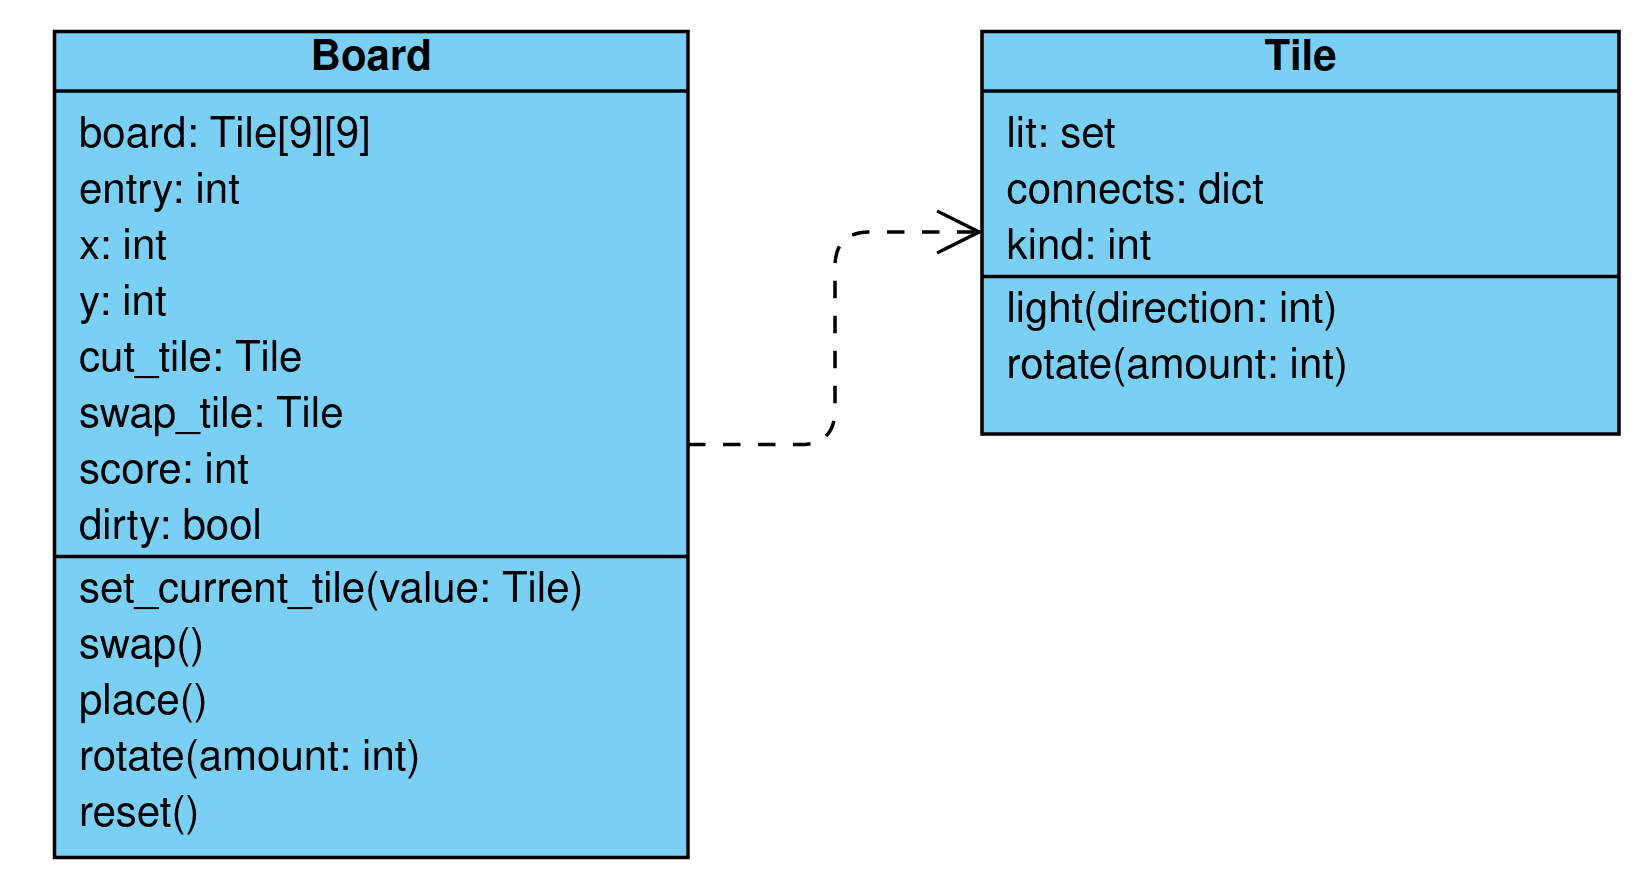
\includegraphics[width=0.68\linewidth]{Figures/board_diagram.png} 
	\caption{Dijagram razreda Board i Tile}
	\label{slk:class_diagram}
\end{figure}
 
Stanje igre određeno je s nekoliko stvari vidljivih na ekranu tijekom igre: 

- koliko ploča jest prazno, ili alternativno, već postavljeno i na kojem mjestu
- gdje nam se nalazi završetak konca; na to mjesto u sljedećem koraku postavljamo novu pločicu
- smjerovi konaca i pozicije svake već do tad postavljene ploče
- izgled zamjenske pločice


\section{Biranje koraka slučajnim odabirom}
\label{pog:slucajan_odabir}

Kako bismo imali nešto s čime dalje možemo uspoređivati efektivnost koje heuristike pogledati će mo što se događa sa igrom ako joj prepustimo odabir svakog sljedećeg koraka slučajnom odabiru. 



%-------------------------------------------------------------------------------
\chapter{Rezultati i rasprava}
\label{pog:rezultati_i_rasprava}

\Blindtext


%--- ZAKLJUČAK / CONCLUSION ----------------------------------------------------
\chapter{Zaključak}
\label{pog:zakljucak}

\blindtext


%--- LITERATURA / REFERENCES ---------------------------------------------------

% Literatura se automatski generira iz zadane .bib datoteke / References are automatically generated from the supplied .bib file
% Upiši ime BibTeX datoteke bez .bib nastavka / Enter the name of the BibTeX file without .bib extension
\bibliography{literatura}



%--- SAŽETAK / ABSTRACT --------------------------------------------------------

% Sažetak na hrvatskom
\begin{sazetak}
  Unesite sažetak na hrvatskom.

  \blindtext
\end{sazetak}

\begin{kljucnerijeci}
  prva ključna riječ; druga ključna riječ; treća ključna riječ
\end{kljucnerijeci}


% Abstract in English
\begin{abstract}
  Enter the abstract in English.
  
  \blindtext 
\end{abstract}

\begin{keywords}
  the first keyword; the second keyword; the third keyword
\end{keywords}


%--- PRIVITCI / APPENDIX -------------------------------------------------------

% Sva poglavlja koja slijede će biti označena slovom i riječi privitak / All following chapters will be denoted with an appendix and a letter
\backmatter

\chapter{The Code}

\Blindtext


\end{document}
